% Tizenegyedik és tizenkettedik előadás

\chapter{Az Intel 2S szerver processzorai}

\section{Bevezetés}
Az Intel szerver processzorai két csoportra oszthatók:
\begin{itemize}
    \item Xeon - x86 alapúak, 2004-től 64 biten
    \item Itanium - VLIW alapúak
\end{itemize}

A továbbiakban a 64 bites Xeonokat vizsgáljuk.
Az első 64 bites 2S szerver processzor a Nocona volt, ami a Pentium 4-re épült.
A Nocona után már minden szerverprocesszor többmagos volt.

Elnevezések: DP - dual processor, MP - multi processzor.
Később ezeket váltották a 2S, 4S és 8S jelölések, amik a foglalatok számára utalnak.
Csak a 2S szerverekkel foglalkozunk.

\subsection{A szerverprocesszorok piaca}
A szerverek nagyrészt 1S és 2S rendszerekre épülnek (91\%).

2005 környéként két jelentős típusú szerver volt forgalomban:
\begin{itemize}
    \item a SUN által képviselt RISC rendszerek
    \item az Intel x86 alapú szerverei
\end{itemize}
Napjainkban gyakorlatilag csak x86 alapú szervereket használunk.

Az Intel és az AMD versenye az évek során:
\begin{figure}[H]
    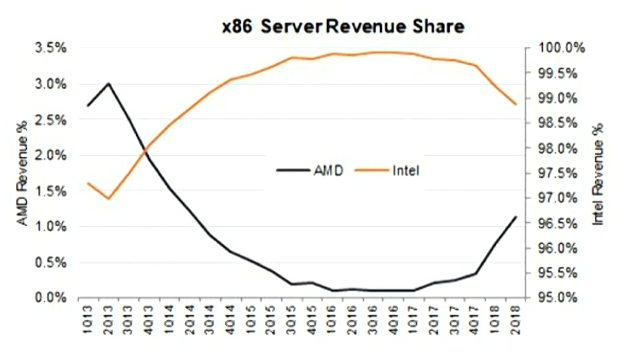
\includegraphics[width=0.8\textwidth]{intelamd}
    \centering
    \caption{Intel és AMD szerver eladások}
    \label{fig:intelamd}
\end{figure}
Az AMD a Zen processzorokkal tudott újra nagyobb részesedést szerezni.
Újdonság, hogy az ARM is bejelentett egy új, szerverorientált családot, a Neoverse-t.
Várható, hogy az ARM processzorok valós konkurenciát fognak jelenteni az AMD-nek és Intelnek.

\subsection{A platform fogalma és a kompatibilitás}
Platformnak tekintjük a rendszer fő komponenseit (a vázát).
Ezek a komponensek:
\begin{itemize}
    \item processzor
    \item chipset
    \item interfészek
\end{itemize}

Egy processzor tehát akkor kompatibilis egy platformmal, ha az adott interfészt támogatja.

\subsection{Szerverplatformok osztályozása}
A platformokat többféleképpen osztályozhatjuk:
\begin{itemize}
    \item foglalatok száma
    \item memória csatolási felület
    \item teljesítmény osztály
    \item lapkakészlet chipeinek száma
\end{itemize}

\subsubsection{Foglalatok száma szerint}
\begin{itemize}
    \item egyprocesszoros
    \item többprocesszoros (2S, 4S, 8S, 8-nál több processzoros)
\end{itemize}

\subsubsection{Az Intel Optane memória}
Az Optane memória egy nem felejtő (non-volatile) memória, ami a memória méretét terjeszti ki, az ezen tárolt adatokat pedig nem kell háttértárra menteni.
Ez egy teljesen új memória technológiát alkalmaz, ez a 3D XPoint, ami a kristályszerkezek különböző állapotait használja ki.

\subsubsection{Memória csatlakozás szerint}
\begin{itemize}
    \item UMA (Uniform Memory Access): azonos elérési időt biztosít minden magnak és processzornak, mivel a memória a memória vezérlő chipre kapcsolódik
    \item NUMA (Non-Uniform Memory Access): a memória a processzorhoz van illesztve, ekkor a processzorok között eltér a memória különböző területeinek az elérése
\end{itemize}
Mindkét esetben minden processzor eléri a teljes memóriaterületet.
NUMA esetében egy adott processzorhoz tartozik lokális (közvetlenül csatlakozó) és távoli memória is.
Távoli memória esetén az elérés egy másik processzorok keresztül történik.

Napjainkban a NUMA technológia dominál.

\subsubsection{Teljesítmény kategória szerint}
Három nagy csoport különböztethető meg:
\begin{itemize}
    \item mainstream
    \item nagyobb teljesítményű
    \item kisebb teljesítményű
\end{itemize}
Az első szerver processzoroknál még nem voltak külön kategóriák, ezeket tekintjük mainstreamnek.

\subsubsection{Chipkészlet chipeinek száma szerint}
\begin{itemize}
    \item két chipet tartalmazó chipkészlet (északi és déli híd)
    \item egy chipes rendszer (a memória és PCI vezérlő a processzorra költözött)
\end{itemize}

\section{Elnevezési rendszerek}
2005-ig az Intel egyszerű elnevezéseket alkalmaztak, a frekvencia és a típus szerint nevezte el a processzorait pl. Intel Xeon 2.8 GHz DP.
Az AMD ekkor a processzorait az alapján nevezte el, hogy az előző generációhoz képest milyen gyorsulást ért el, pl. AMD Athlon 1600+.

Később az Intel áttért az AMD-hez hasonló nevezékekre, a relatív teljesítmény alapján megjelentek a 3000-es, 5000-es, 7000-es és 9000-es processzorok.
A probléma ezzekkel a nevekkel, hogy nem sokat mondanak el a teljesítményről, ezért ezután az EX (Expandable, nagy teljesítményű), EP (Efficient performance, mainstream) és az EN (Entry level, belépőszint) jelölésekkel látta el a processzorait.
2011-ben egy részletesebb elnevezési sémát vezetett be az Intel.

Erre egy példa: Intel Xeon E7-4820 v2.
Az E(3/5/7) a termékcsaládot jelenti, összhangban a desktopok i3, i5, i7 rendszereivel.
A példában a 4-es szám megadja, hogy hány processzort támogat a rendszer.
A 8-as szám a socket típust jelöli, ami valójában a teljesítmény kategóriának felel meg (4=EN, 6=EP vagy 8=EX).
A 2-es a processzor SKU-ját (Storage Keeping Unit) jelenti, ami gyakorlatilag a modellszám.
Végül a v2 a verziószám, a Sandy Bridge volt az első verzió, ezt még nem jelölték külön.
A v2 tehát egy Ivy Bridge processzor.
Ezek közben az Itanium elnevezése nem változott.

Az EX, EP és EN platformok több szempontból is eltérnek egymástól:
\begin{itemize}
    \item memória csatolás módja
    \item rendszer linkek száma
    \item memória csatornák száma
    \item PCIe vonalpárok száma
\end{itemize}

Az Intel legújabb elnevezési rendszere a Skylake családdal mutatkozott be, 2017-ben.
Az új processzorcsalád egy skálázható koncepciót követ:
\begin{itemize}
    \item egységesíti a processzorok felépítését a támogatott foglalatok számától függetlenül
    \item négy teljesítmény kategóriát vezet be az E5 és E7 helyett, az E3-at pedig megszüntetik
\end{itemize}
Az új teljesítmény kategóriák:
\begin{itemize}
    \item Platinum
    \item Gold
    \item Silver
    \item Bronze
\end{itemize}
A különböző osztályok különböző mennyiségű processzort támogatnak.
Az új 4 számjegyű jelölési rendszer pedig a következő ábrán látható.
\begin{figure}[H]
    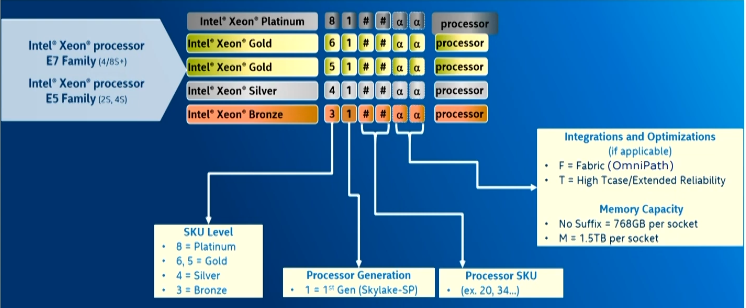
\includegraphics[width=0.8\textwidth]{naming}
    \centering
    \caption{Az Intel legújabb szerver processzor nevezéktana}
    \label{fig:naming}
\end{figure}

\section{Processzorok fejlődése}
Az első Intel 64 bites szerver processzor még egy magos volt (Nocona).
A fejlődés során három fő fázis különböztethető meg:
\begin{itemize}
    \item dedikált szerver processzorok 2S és 4S konfigurációkhoz (2004-2007)
    \item piaci szegmens specifikus processzorok (EN, EP, EX), ezek már mind NUMA processzorok (2010-2016)
    \item skálázható szerver platformok (2017-)
\end{itemize}

A fejlődést négy szempont szerint vizsgálhatjuk:
\begin{itemize}
    \item memóriacsatlakozás (UMA, NUMA)
    \item platform kialakítás (dedikált, szegmens orientált, skálázható)
    \item teljesítmény kategória
    \item támogatott processzorok száma 
\end{itemize}
Először az UMA rendszerek jelentek meg, amik 2 vagy 4 processzort támogattak és dedikált platformnak számítottak.
Következő lépcsőben NUMA rendszerekről beszélhetünk, amik szegmens orientáltak voltak és 3 különböző teljesítmény osztályban készültek, legfeljebb 8 támogatott processzorral
Végül a skálázható platformok jelentek meg, de az Intel közben bejelentett két dedikált processzort.

\section{A memória alrendszerek tervezési kihívásai}
A szerver processzorok fejlődésének első fázisában a magok száma körülbelül két évente duplázódott.
Ez összhangban volt Moore törvényével.
A folyamat akkor változott meg, amikor az L3 cache-ek megjelentek, amik nagyon nagy részét lefoglalták a tranzisztoroknak.
Következmény, hogy a magok számának duplázódása lelassult, már nagyjából 4 év kellett hozzá.
Itt már eltér a fejlődés a Moore szabálytól, mivel a processzor lapka méretét nem tudták arányosan növelni a növekvő gyártási hibaarány miatt (emiatt a hűtés problémásabb volt, a tranzisztorok összezsúfolódtak, a disszipáció korlátozta a tranzisztorok növekedését).
A következő torpanás a 10 nm-es technológia kifejlesztésénél jött, de utána visszatért a 4 évenkénti duplázódás.

A memóriák ezzel szemben 8 évente duplázták a teljesítményüket.
A magszámok tehát sokkal gyorsabban nőttek, mint a memória gyorsasága.
Az egy magra jutó memória sávszélesség viszont meghatározó a rendszer összteljesítményénél, ideális esetben ez a generációk között konstans marad, hogy ne jelentsen szűk keresztmetszetet a memória.
A memóriák sebbessége viszont nem tudta tartani a lépést, ezért a memória csatornák számát kellett növelni az arány fenntartása érdekében.

Megfigyelték, hogy egy adott magszámhoz hány memóriacsatorna szükséges: 2 magnál még elég 2 csatorna, 32 magos rendszerek esetén viszont már 8 csatornára van szükség.
Probléma, hogy a csatornák számának növelése technikailag nagyon nehéz (több vezeték kell, megjelennek az áthallások, stb.).

\section{Skálázható 2S Intel szerver processzorok}
A skálázható szerver processzorok a fejlődés harmadik fázisát jelentik.
Az Intel két skálázható processzorcsaládja a Purley (Skylake, Cascade lake alapok) és a Whitley (Ice lake alapok).
Ezek mind NUMA processzorok.
A Purley Platinum processzorok 1-8, a Goldok 1-4, a Silver és a Bronze osztályú processzorok pedig 1-2 processzort támogatnak.
A Whitley család viszont legfeljebb 2 processzorig skálázható, ezért ez nem is igazán számít skálázhatónak.

A Purley platformot 2017-ben jelentették be, 10 nm technológiával készül.
Fő célja az adatközponti, felhő és mesterséges intelligencia felhasználások támogatása.
Fontos, hogy egységesíti a processzorok tervezését, a 2S, 4S és 8S konfigurációk azonos elemekből építkeznek.

\subsection{Teljesítmény}
A Skylake az Intel kétfázisú fejlesztési ciklusában a Tock fázisba esik, tehát új architektúrát jelent és kb. 10\%-os teljesítmény növekedést hozott.
Ha a 2006-ban megjelent Core 2 szerver processzorokhoz hasonlítjuk a Purley (Skylake) CPU-kat, többszálas teljesítményben kb. 41-szeres növekedést értek el.
A SPECint egyszálas benchmark szerint 3,8-szoros a teljesítmény.
A többszálas végrehajtás nagyon nagy mértékben nőtt a növekvő magszám miatt.

\subsection{Interconnect}
A Broadwell processzorok adatgyűrűs adatkapcsolati megoldással rendelkeznek, ez a megoldás viszont a magszám növekedésével egyre komplexebbé vált, csökkent a hatékonysága.
Ezért a Skylake-nál egy 2D-s adatkapcsolati réteg jelent meg, ahol az adatok csomagokban közlekednek.
Ez a váltás nagyban hozzájárult a rendszer gyorsulásához.

\subsection{A Skylake-et követő architektúrák}
A Skylake-el az Intel áttért egy három fázisú fejlesztési modellre a korábbi tick-tock helyett.
Az első fázisban megtörténik a technológiai váltás (csíkszélesség csökkentése), ezt követi az új mikroarchitektúra, majd ezt követően több lépésben optimalizálják a mikroarchitektúrát.

\subsection{A Cascade Lake szerver processzorok}
A Cascade Lake alapú Purley processzorok a skálázható Skylake CPU-k optimalizálása.
A Cascade Lake-en belül két sorozat létezik: SP és AP.
Míg az SP a hagyományos rendszer, az AP két lapkát integrál egy tokban.

\subsubsection{SP vonal}
Az SP 2019-ben jelent meg, legfeljebb 28 magot támogat.
14++ nm-es technológiával készült, ami a 14 nm-es optimalizált változata.
Sokban nem különbözik az előző rendszerre, viszont tartalmaz több optimalizációt és új neurális kiterjesztéseket vezet be.

Újítás még az Optane memória támogatása és biztonsági javítások.

\subsubsection{AP vonal}
Az AP 2x28, azaz 56 magot alkalmaz, csak a Platinum kategóriás processzorok valósítják meg.
Forrasztandó tokozással érkezik.

Elsősorban nagy számítási igényű alkalmazásokhoz, mesterséges intelligenciához vagy IaaS megoldásokhoz ajánlják.
Csak OEM-ek számára eladó, csak teljes eszköz formájában (számítási modulok).
Méretre kimondottan nagy a processzor, 76x76 mm.

A támogatott memória mennyisége és sebessége is megnőtt a Skylake-hez képest.
Itt is megjelent az Optane memória, az új utasítás kiterjesztés és a biztonsági javítások.

Két ilyen processzor megfelelően összekötve már egy négy processzoros rendszert ad.

\subsection{A Whitley szerver processzorok}
A Whitley a Purley-t követő processzorcsalád.
2021 áprilisában jelent meg, 10 nm-es technológiára épül.

Az Intel skálázható szerver platformként árulja, de a Whitley csak 1 és 2 processzort támogat, a 4-8 processzoros rendszerekhez külön család tartozik, ez a Cedar Island.
Tehát ez nem teljesen skálázható, csak egy szükségmegoldás.
A Purley valódi utódja még nem jelent meg.

\subsubsection{A Whitley (Ice Lake) újításai}
Az előző generáció 6 memóriacsatornája helyett 8-al rendelkezik, ami indokolt is, mivel max. 40 magot támogat a 28 helyett.
Növekedett a ROB mérete, a regiszterfájlok és a cache-ek méretei is.

\subsubsection{Konkurencia}
Az Intel Ice Lake processzorai lemaradtak az AMD és az Altra rendszereitől.